
\chapter{Publish on the server}
\label{chap:publish}

%\nomenclature{SP1}{Service pack 1}
In this appendix are step-by-step instructions how to publish the web site on the Windows Server 2008 R2 Standard x64 SP1.
At the end of this chapter is mentioned the migration of the server.

\section{Creation of publish package}
\label{sec:deployPackage}


\subsection{Settings}

The web should be configured before the first deploy.
The configuration settings are in the \emph{Web.config} file and they are explained in \autoref{sec:configWorkDir}.

The most settings can be left as default but at leas a valid keys for the \emph{ReCaptcha} should be set [\ref{sec:reCaptcha}].
Also correct ID for \emph{Google Analytics} [\ref{sec:ga}] can be set in the Layout view (\emph{/Views/Shared/\_Layout.cshtml}).


\subsection{Compilation}

Creation of the publish package is simple.
Open the solution in the Visual Studio 2010 and in the \emph{Solution explorer} right click on the \emph{Malsys.Web} project and chose \emph{Publish} from the context menu (Fig. \ref{fig:publishVs}).
Then appears a popup dialog with publish settings.
In this tutorial we will use publishing to the file system as you can see in \autoref{fig:publishDialog}.
Then click on the \emph{Publish} button and the publish package will be created in selected directory.
Do not forget to set \emph{release} configuration in the Visual Studio 2010 before publishing.

\begin{figure}[h!]
	\subfloat[]{\label{fig:publishVs}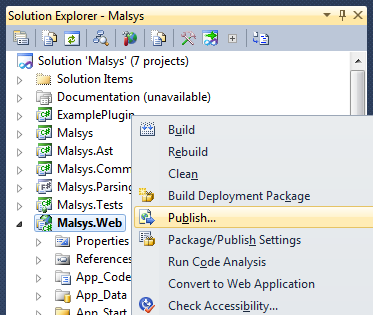
\includegraphics[width=0.5\linewidth]{PublishVs}}
	\hfill
	\subfloat[]{\label{fig:publishDialog}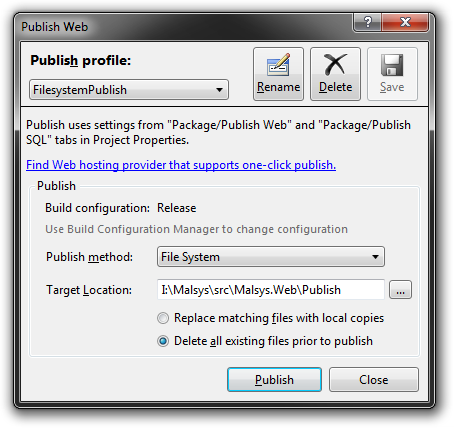
\includegraphics[width=0.46\linewidth]{PublishDialog}}
	\caption{Creation of publish the package in the Visual Studio 2010}
	\label{fig:publish}
\end{figure}
 
 

\section{Configuration of the server}

Following steps expects fresh installation of the Windows Server 2008 R2 Standard x64 SP1.
Any step can be skipped if any described component is already installed.


\subsection{Internet Information Services (IIS)}

To run the web we will need the IIS on the server.

To install it, run the \emph{Server Manager} and in \emph{Roles summary} click on the \emph{Add Roles} button.
Skip the \emph{Before You Begin} page if it appears, select the \emph{Web Server (IIS)} from the list and click the \emph{Next} button.
On \emph{Role Services} screen select \emph{ASP.NET} and \emph{HTTP Redirection} and confirm installation of any dependencies as well.
Then click the \emph{Next} button and finish installation.


\subsection{Web platform installer}

For installation of needed programs we will use the Web platform installer.

Download the \emph{Web Platform Installer} from \url{http://www.microsoft.com/web/downloads/platform.aspx} and run it.
In the \emph{Web Platform Installer} switch to the \emph{Products} tab and mark to install following products (\autoref{fig:wpi}):
\begin{itemize*}
	\item Microsoft .NET Framework 4
	\item SQL Server Express 2008 R2
	\item ASP.NET MVC 3 (Visual Studio 2010)
	\item ASP.NET WebPages
	\item ASP.NET MVC Tools Update
	\item ASP.NET Web Pages Language Packs Language Packs
	\item URL Rewrite 2.0
	\item IIS: Logging Tools
\end{itemize*}

\begin{figure}[h!]
	\centering
	\subfloat{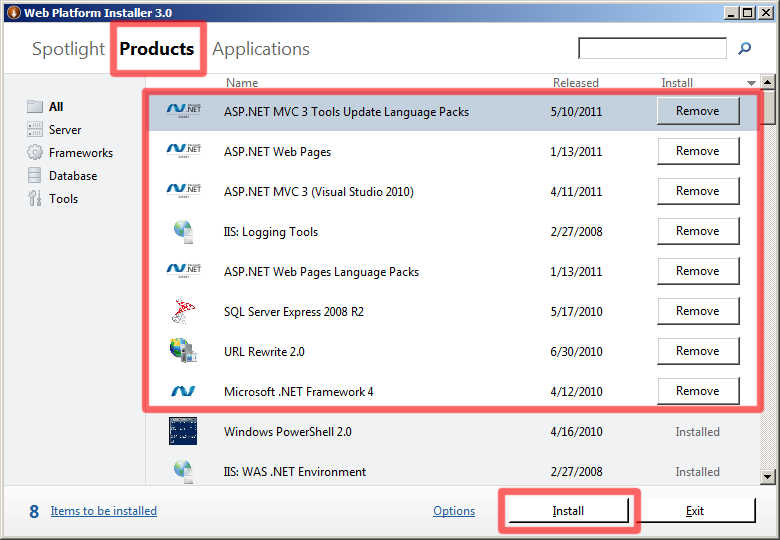
\includegraphics[width=0.8\linewidth]{WebPlatformInstaller}}
	\caption{Marked products to install in the \emph{Web Platform Installer}}
	\label{fig:wpi}
\end{figure}
		
		

\subsection{F\#}

\subsubsection{F\# Redistributable Package}

To load the F\# 4.0 libraries properly the \emph{F\# 2.0 Runtime SP1} must be installed.
The redistributable package can be downloaded from \url{http://msdn.microsoft.com/en-us/library/ee829875.aspx}.

\subsubsection{F\# PowerPack}

Standard F\# distribution do not contain tolls like FsLex and FsYacc which are used in this project.
They are in downloadable package called the \emph{F\# PowerPack} which can be downloaded from \url{http://fsharppowerpack.codeplex.com/}.


\section{Deploy of the application}

In this moment all needed software to run the web is installed on the server.


\subsection{Creation of new Application pool}

For running the web we will create a new Application pool (App pool) because default App pools are not configured as we need.

Open the \emph{Internet Information Services (IIS) Manager}\footnote{The \emph{Internet Information Services (IIS) Manager} can be easily found typing the "IIS" in the start menu search bar.}, in the left menu open tree node with the name of your server, right click on the \emph{Application Pools} and choose the \emph{Add Application Pool} from the context menu.
Enter the name (\emph{Malsys} in our case) of new App pool and as the \emph{.NET Framework version} chose \emph{.NET Framework v4.0} (Fig. \ref{fig:newAppPool}) and confirm the dialog.

Then select \emph{Application Pools} node (left menu), right click on newly created App pool and chose \emph{Advanced settings}.
In the \emph{Advanced Settings} dialog box find the category called \emph{Process Model}.
The first row in the category will be the \emph{Identity} row.
Click on the \emph{Identity} row and then click on the small button that shows on the right-hand side of the value cell.
A dialog box called \emph{Application Pool Identity} will popup.
Within that dialog box make sure the first radio button titled \emph{Built-in Account} is selected.
In the dropdown box below the radio button choose \emph{Network Service} for the identity (Fig. \ref{fig:appPoolSettings}).
Then confirm all dialogs with \emph{Ok} buttons.

\begin{figure}[h!]
	\subfloat[New app pool dialog]{
		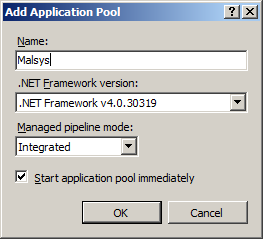
\includegraphics[width=0.4\linewidth]{NewAppPool}
		\label{fig:newAppPool}
	} \hfill
	\subfloat[App pool settings dialog]{
		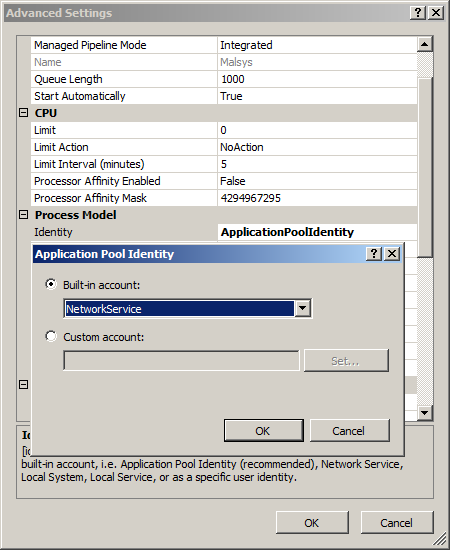
\includegraphics[width=0.5\linewidth]{AppPoolSettings}
		\label{fig:appPoolSettings}
	}
	\caption{App pool settings dialogs}
\end{figure}


\subsection{Creation of new App Pool}

In the \emph{Internet Information Services (IIS) Manager} click on \emph{Sites} node on the left menu.
If your installation of the IIS is fresh you can delete the default site called \emph{Default Site}.
Then right click \emph{Sites} node and chose \emph{Add Web Site}.

In the dialog, enter the \emph{Site name} and chose newly created App pool from previous step.
Then enter physical path of the web root (\emph{C:\textbackslash{}inetpub\textbackslash{}WwwMalsys} in our case).
Then you can configure \emph{Binding}.
If the server will host only this web site we can leave default settings (Fig. \ref{fig:addWebSite}).

\begin{figure}[h!]
	\centering
	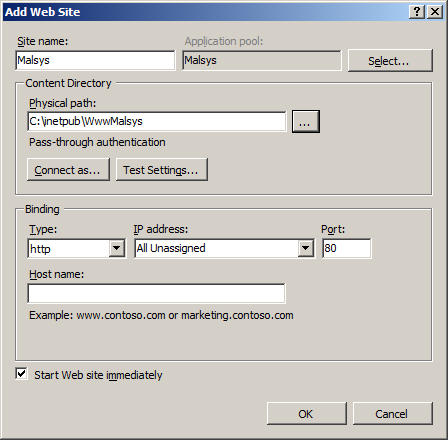
\includegraphics[width=0.6\linewidth]{WebSite}
	\caption{Filled \emph{Add Web Site} dialog}	
	\label{fig:addWebSite}
\end{figure}


\subsection{Copy files}


Copy all files from the deployment package (created in \autoref{sec:deployPackage}) to the web site root.
Database file is not included in deployment package to avoid rewriting "life" version while updating the web site.
Empty database file is located in the \emph{App\_Data.empty.zip} archive in the \emph{App\_Data} directory of the \emph{Malsys.Web} project.
Extract both files from the archive to the \emph{App\_Data} directory of the new web.

To allow access of database server to the database files set access to the \emph{App\_Data} to full control for users \emph{NETWORK SERVICE} and \emph{IIS\_IUSRS} as you can see in \autoref{fig:appDataRights}.

\begin{figure}[h!]
	\centering
	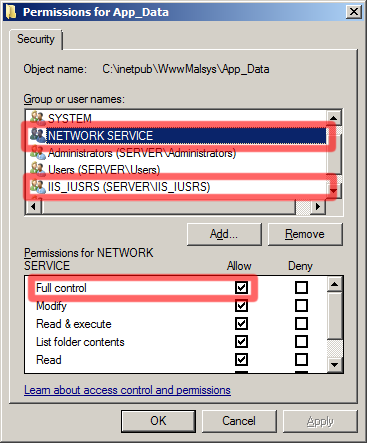
\includegraphics[width=0.45\linewidth]{AppDataRights}
	\caption{Rights of the \emph{App\_Data} directory}
	\label{fig:appDataRights}
\end{figure}
	

\section{First run}

The web has detection for correctness of basic settings.
One of them are working directories for processing and gallery configurable in the \emph{Web.config} (see \autoref{sec:configWorkDir}).
They must be created and accessible for reading and writing for the \emph{IIS\_IUSRS} user in order to run the web.
The web application will try to create them but if it fail an exception is thrown.
The same applies for directory for logging of errors which is also settable in the \emph{Web.config}.

The database is also checked.
The existence of following user roles is checked: \emph{administrator}, \emph{trusted}, \emph{viewstats} and \emph{viewfeedbacks}.
Missing ones are recreated.

If there is no user in the DB a new user with name \emph{Administrator} is created and automatically added to the \emph{administrator} role.
This user have password set to \emph{malsys}.
This is important because without administrator is not possible to add any users to user roles, thus it is not possible to promote any user to new administrator.
The password of this default user should be changed immediately after deploying.



\section{Server migration}

The migration of the server is very simple.
If the new server is prepared all what needs to be done is transfer of the database.
Since DB is stored in single \emph{.mdf} file it can be just copied and that's it. 

Each image in the gallery will generate automatically on the first request for it.

















